% Options for packages loaded elsewhere
\PassOptionsToPackage{unicode}{hyperref}
\PassOptionsToPackage{hyphens}{url}
\PassOptionsToPackage{dvipsnames,svgnames,x11names}{xcolor}
%
\documentclass[
  letterpaper,
  DIV=11,
  numbers=noendperiod]{scrartcl}

\usepackage{amsmath,amssymb}
\usepackage{lmodern}
\usepackage{iftex}
\ifPDFTeX
  \usepackage[T1]{fontenc}
  \usepackage[utf8]{inputenc}
  \usepackage{textcomp} % provide euro and other symbols
\else % if luatex or xetex
  \usepackage{unicode-math}
  \defaultfontfeatures{Scale=MatchLowercase}
  \defaultfontfeatures[\rmfamily]{Ligatures=TeX,Scale=1}
\fi
% Use upquote if available, for straight quotes in verbatim environments
\IfFileExists{upquote.sty}{\usepackage{upquote}}{}
\IfFileExists{microtype.sty}{% use microtype if available
  \usepackage[]{microtype}
  \UseMicrotypeSet[protrusion]{basicmath} % disable protrusion for tt fonts
}{}
\makeatletter
\@ifundefined{KOMAClassName}{% if non-KOMA class
  \IfFileExists{parskip.sty}{%
    \usepackage{parskip}
  }{% else
    \setlength{\parindent}{0pt}
    \setlength{\parskip}{6pt plus 2pt minus 1pt}}
}{% if KOMA class
  \KOMAoptions{parskip=half}}
\makeatother
\usepackage{xcolor}
\setlength{\emergencystretch}{3em} % prevent overfull lines
\setcounter{secnumdepth}{-\maxdimen} % remove section numbering
% Make \paragraph and \subparagraph free-standing
\ifx\paragraph\undefined\else
  \let\oldparagraph\paragraph
  \renewcommand{\paragraph}[1]{\oldparagraph{#1}\mbox{}}
\fi
\ifx\subparagraph\undefined\else
  \let\oldsubparagraph\subparagraph
  \renewcommand{\subparagraph}[1]{\oldsubparagraph{#1}\mbox{}}
\fi

\usepackage{color}
\usepackage{fancyvrb}
\newcommand{\VerbBar}{|}
\newcommand{\VERB}{\Verb[commandchars=\\\{\}]}
\DefineVerbatimEnvironment{Highlighting}{Verbatim}{commandchars=\\\{\}}
% Add ',fontsize=\small' for more characters per line
\usepackage{framed}
\definecolor{shadecolor}{RGB}{241,243,245}
\newenvironment{Shaded}{\begin{snugshade}}{\end{snugshade}}
\newcommand{\AlertTok}[1]{\textcolor[rgb]{0.68,0.00,0.00}{#1}}
\newcommand{\AnnotationTok}[1]{\textcolor[rgb]{0.37,0.37,0.37}{#1}}
\newcommand{\AttributeTok}[1]{\textcolor[rgb]{0.40,0.45,0.13}{#1}}
\newcommand{\BaseNTok}[1]{\textcolor[rgb]{0.68,0.00,0.00}{#1}}
\newcommand{\BuiltInTok}[1]{\textcolor[rgb]{0.00,0.23,0.31}{#1}}
\newcommand{\CharTok}[1]{\textcolor[rgb]{0.13,0.47,0.30}{#1}}
\newcommand{\CommentTok}[1]{\textcolor[rgb]{0.37,0.37,0.37}{#1}}
\newcommand{\CommentVarTok}[1]{\textcolor[rgb]{0.37,0.37,0.37}{\textit{#1}}}
\newcommand{\ConstantTok}[1]{\textcolor[rgb]{0.56,0.35,0.01}{#1}}
\newcommand{\ControlFlowTok}[1]{\textcolor[rgb]{0.00,0.23,0.31}{#1}}
\newcommand{\DataTypeTok}[1]{\textcolor[rgb]{0.68,0.00,0.00}{#1}}
\newcommand{\DecValTok}[1]{\textcolor[rgb]{0.68,0.00,0.00}{#1}}
\newcommand{\DocumentationTok}[1]{\textcolor[rgb]{0.37,0.37,0.37}{\textit{#1}}}
\newcommand{\ErrorTok}[1]{\textcolor[rgb]{0.68,0.00,0.00}{#1}}
\newcommand{\ExtensionTok}[1]{\textcolor[rgb]{0.00,0.23,0.31}{#1}}
\newcommand{\FloatTok}[1]{\textcolor[rgb]{0.68,0.00,0.00}{#1}}
\newcommand{\FunctionTok}[1]{\textcolor[rgb]{0.28,0.35,0.67}{#1}}
\newcommand{\ImportTok}[1]{\textcolor[rgb]{0.00,0.46,0.62}{#1}}
\newcommand{\InformationTok}[1]{\textcolor[rgb]{0.37,0.37,0.37}{#1}}
\newcommand{\KeywordTok}[1]{\textcolor[rgb]{0.00,0.23,0.31}{#1}}
\newcommand{\NormalTok}[1]{\textcolor[rgb]{0.00,0.23,0.31}{#1}}
\newcommand{\OperatorTok}[1]{\textcolor[rgb]{0.37,0.37,0.37}{#1}}
\newcommand{\OtherTok}[1]{\textcolor[rgb]{0.00,0.23,0.31}{#1}}
\newcommand{\PreprocessorTok}[1]{\textcolor[rgb]{0.68,0.00,0.00}{#1}}
\newcommand{\RegionMarkerTok}[1]{\textcolor[rgb]{0.00,0.23,0.31}{#1}}
\newcommand{\SpecialCharTok}[1]{\textcolor[rgb]{0.37,0.37,0.37}{#1}}
\newcommand{\SpecialStringTok}[1]{\textcolor[rgb]{0.13,0.47,0.30}{#1}}
\newcommand{\StringTok}[1]{\textcolor[rgb]{0.13,0.47,0.30}{#1}}
\newcommand{\VariableTok}[1]{\textcolor[rgb]{0.07,0.07,0.07}{#1}}
\newcommand{\VerbatimStringTok}[1]{\textcolor[rgb]{0.13,0.47,0.30}{#1}}
\newcommand{\WarningTok}[1]{\textcolor[rgb]{0.37,0.37,0.37}{\textit{#1}}}

\providecommand{\tightlist}{%
  \setlength{\itemsep}{0pt}\setlength{\parskip}{0pt}}\usepackage{longtable,booktabs,array}
\usepackage{calc} % for calculating minipage widths
% Correct order of tables after \paragraph or \subparagraph
\usepackage{etoolbox}
\makeatletter
\patchcmd\longtable{\par}{\if@noskipsec\mbox{}\fi\par}{}{}
\makeatother
% Allow footnotes in longtable head/foot
\IfFileExists{footnotehyper.sty}{\usepackage{footnotehyper}}{\usepackage{footnote}}
\makesavenoteenv{longtable}
\usepackage{graphicx}
\makeatletter
\def\maxwidth{\ifdim\Gin@nat@width>\linewidth\linewidth\else\Gin@nat@width\fi}
\def\maxheight{\ifdim\Gin@nat@height>\textheight\textheight\else\Gin@nat@height\fi}
\makeatother
% Scale images if necessary, so that they will not overflow the page
% margins by default, and it is still possible to overwrite the defaults
% using explicit options in \includegraphics[width, height, ...]{}
\setkeys{Gin}{width=\maxwidth,height=\maxheight,keepaspectratio}
% Set default figure placement to htbp
\makeatletter
\def\fps@figure{htbp}
\makeatother

\KOMAoption{captions}{tableheading}
\makeatletter
\makeatother
\makeatletter
\makeatother
\makeatletter
\@ifpackageloaded{caption}{}{\usepackage{caption}}
\AtBeginDocument{%
\ifdefined\contentsname
  \renewcommand*\contentsname{Table of contents}
\else
  \newcommand\contentsname{Table of contents}
\fi
\ifdefined\listfigurename
  \renewcommand*\listfigurename{List of Figures}
\else
  \newcommand\listfigurename{List of Figures}
\fi
\ifdefined\listtablename
  \renewcommand*\listtablename{List of Tables}
\else
  \newcommand\listtablename{List of Tables}
\fi
\ifdefined\figurename
  \renewcommand*\figurename{Figure}
\else
  \newcommand\figurename{Figure}
\fi
\ifdefined\tablename
  \renewcommand*\tablename{Table}
\else
  \newcommand\tablename{Table}
\fi
}
\@ifpackageloaded{float}{}{\usepackage{float}}
\floatstyle{ruled}
\@ifundefined{c@chapter}{\newfloat{codelisting}{h}{lop}}{\newfloat{codelisting}{h}{lop}[chapter]}
\floatname{codelisting}{Listing}
\newcommand*\listoflistings{\listof{codelisting}{List of Listings}}
\makeatother
\makeatletter
\@ifpackageloaded{caption}{}{\usepackage{caption}}
\@ifpackageloaded{subcaption}{}{\usepackage{subcaption}}
\makeatother
\makeatletter
\@ifpackageloaded{tcolorbox}{}{\usepackage[many]{tcolorbox}}
\makeatother
\makeatletter
\@ifundefined{shadecolor}{\definecolor{shadecolor}{rgb}{.97, .97, .97}}
\makeatother
\makeatletter
\makeatother
\ifLuaTeX
  \usepackage{selnolig}  % disable illegal ligatures
\fi
\IfFileExists{bookmark.sty}{\usepackage{bookmark}}{\usepackage{hyperref}}
\IfFileExists{xurl.sty}{\usepackage{xurl}}{} % add URL line breaks if available
\urlstyle{same} % disable monospaced font for URLs
\hypersetup{
  pdftitle={Problem Set 2},
  pdfauthor={Sam Turner},
  colorlinks=true,
  linkcolor={blue},
  filecolor={Maroon},
  citecolor={Blue},
  urlcolor={Blue},
  pdfcreator={LaTeX via pandoc}}

\title{Problem Set 2}
\author{Sam Turner}
\date{September 28, 2022}

\begin{document}
\maketitle
\ifdefined\Shaded\renewenvironment{Shaded}{\begin{tcolorbox}[breakable, enhanced, interior hidden, frame hidden, borderline west={3pt}{0pt}{shadecolor}, sharp corners, boxrule=0pt]}{\end{tcolorbox}}\fi

\hypertarget{theory-and-concepts}{%
\section{Theory and Concepts}\label{theory-and-concepts}}

\hypertarget{question-1}{%
\subsection{Question 1}\label{question-1}}

In your own words, explain the difference between endogeneity and
exogeneity.

A factor, x, is exogenous if it does not affect any other factors which
affect some factor y. This means that the factor x is either directly
influential on y, or is completely independent.

A factor x is said to be endogenous if it affects any other factor the
is related to some factor y. This means that a factor x is endogenous if
has any affect on some factor z, which affects the factor y. Even if the
factor x is also a direct factor of y.

\hypertarget{question-2}{%
\subsection{Question 2}\label{question-2}}

\hypertarget{part-a}{%
\subsubsection{Part A}\label{part-a}}

In your own words, explain what (sample) standard deviation *means*.

A sample standard deviation is a measurement of much variance from the
mean there is in a given sample of a population.

\hypertarget{part-b}{%
\subsubsection{Part B}\label{part-b}}

In your own words, explain how (sample) standard deviation \emph{is
calculated}. You may also write the formula, but it is not necessary.

Sample standard deviation is calculated by taking the square root of the
variance divided by the correcting term n-1, where n is the sample size.
The variance is calculated by first taking the mean of the sample. Then,
square the difference of between each value in the sample and the sample
mean. Finally, sum the squared values and you have the variance in a
given sample.

\hypertarget{problems}{%
\section{Problems}\label{problems}}

For the remaining questions, you may use \texttt{R} to \emph{verify},
but please calculate all sample statistics by hand and show all work.

\hypertarget{question-3}{%
\subsection{Question 3}\label{question-3}}

Suppose you have a very small class of four students that all take a
quiz. Their scores are reported as follows:

\[\{83, 92, 72, 81 \}
\]

\hypertarget{part-a-1}{%
\subsubsection{Part A}\label{part-a-1}}

Calculate the median.

Because the sample size is even (n=4), we must take the arithmetic mean
of the remaining two median numbers, 81 and 83. The arithmetic mean of
these two numbers is 82.

(81+83)/2 = 164/2 = 82

\hypertarget{part-b-1}{%
\subsubsection{Part B}\label{part-b-1}}

Calculate the sample mean, \(\bar{x}\).

The sample mean is the simply the sum of the sample values divided by
the number of values:

(83+92+72+81) / 4 = 328 / 4 = 82

\hypertarget{part-c}{%
\subsubsection{Part C}\label{part-c}}

Calculate the sample standard deviation, \(s\).

To begin we need to calculate the sample standard deviation, which we
have done above and know it is 82.

We then need to calculate how far each of the given values are from the
mean:

(83-82, 92-82, 72-82, 81-82) = (1, 10, -10, 1).

And then square those differences:

(1, 100, 100, 1).

Sample variance is calculated by taking the sum of these squared
differences and dividing it by n-1 where n is the sample size:

(1+100+100+1) / 4-1 = 202 / 3 = 67.33.

Finally, the sample standard deviation is simply the square-root of the
sample variance. Which is the square-root of 67.33 and is roughly equal
to 8.206.

To help with visualization I have included some code:

\begin{Shaded}
\begin{Highlighting}[]
\FunctionTok{library}\NormalTok{(tidyverse)}
\end{Highlighting}
\end{Shaded}

\begin{verbatim}
-- Attaching packages --------------------------------------- tidyverse 1.3.2 --
v ggplot2 3.3.6     v purrr   0.3.4
v tibble  3.1.8     v dplyr   1.0.9
v tidyr   1.2.0     v stringr 1.4.1
v readr   2.1.2     v forcats 0.5.2
-- Conflicts ------------------------------------------ tidyverse_conflicts() --
x dplyr::filter() masks stats::filter()
x dplyr::lag()    masks stats::lag()
\end{verbatim}

\begin{Shaded}
\begin{Highlighting}[]
\NormalTok{quiz\_score }\OtherTok{\textless{}{-}} \FunctionTok{tibble}\NormalTok{(}\AttributeTok{score =} \FunctionTok{c}\NormalTok{(}\DecValTok{83}\NormalTok{, }\DecValTok{92}\NormalTok{, }\DecValTok{72}\NormalTok{, }\DecValTok{81}\NormalTok{))}

\NormalTok{quiz\_score }\OtherTok{\textless{}{-}}\NormalTok{ quiz\_score }\SpecialCharTok{\%\textgreater{}\%} 
  \FunctionTok{mutate}\NormalTok{(}\AttributeTok{dif =}\NormalTok{ score }\SpecialCharTok{{-}} \DecValTok{82}\NormalTok{) }\SpecialCharTok{\%\textgreater{}\%} 
  \FunctionTok{mutate}\NormalTok{(}\AttributeTok{dif\_sqr =}\NormalTok{ dif}\SpecialCharTok{**}\DecValTok{2}\NormalTok{)}

\NormalTok{quiz\_score}
\end{Highlighting}
\end{Shaded}

\begin{verbatim}
# A tibble: 4 x 3
  score   dif dif_sqr
  <dbl> <dbl>   <dbl>
1    83     1       1
2    92    10     100
3    72   -10     100
4    81    -1       1
\end{verbatim}

\hypertarget{part-d}{%
\subsubsection{Part D}\label{part-d}}

Make or sketch a rough histogram of this data, with the size of each bin
being 10 (i.e.~70's, 80's, 90's, 100's). You can draw this by hand or
use \texttt{R}.

If you are using \texttt{ggplot}, you want to use
\texttt{+\ geom\_histogram(breaks\ =\ seq(start,end,by))} and add
another layer \texttt{+\ scale\_x\_continuous(breaks=seq(start,end,by))}
. The first layer creates bins in the histogram, and the second layer
creates ticks on the x axis; both by creating a \texttt{seq}uence
starting at some \texttt{start}ing value, some \texttt{end}ing value,
\texttt{by} a certain interval (e.g.~by 2, or by 10).\\
\strut \\
Is this distribution roughly symmetric or skewed? What would we expect
about the mean and the median?

As we can see below, the data does not appear to be skewed. We can
verify this finding because we know that the median=mean since we solved
for both above.

\begin{Shaded}
\begin{Highlighting}[]
\CommentTok{\# write your code here!}
\FunctionTok{ggplot}\NormalTok{(}\AttributeTok{data =}\NormalTok{ quiz\_score, }\FunctionTok{aes}\NormalTok{(}\AttributeTok{x=}\NormalTok{score))}\SpecialCharTok{+}
  \FunctionTok{geom\_histogram}\NormalTok{(}\AttributeTok{breaks =} \FunctionTok{seq}\NormalTok{(}\DecValTok{70}\NormalTok{, }\DecValTok{100}\NormalTok{, }\DecValTok{10}\NormalTok{), }\AttributeTok{fill=}\StringTok{"brown"}\NormalTok{, }\AttributeTok{color=}\StringTok{"black"}\NormalTok{)}\SpecialCharTok{+}
  \FunctionTok{scale\_x\_continuous}\NormalTok{(}\AttributeTok{breaks =} \FunctionTok{seq}\NormalTok{(}\DecValTok{70}\NormalTok{, }\DecValTok{100}\NormalTok{, }\DecValTok{10}\NormalTok{))}
\end{Highlighting}
\end{Shaded}

\begin{figure}[H]

{\centering 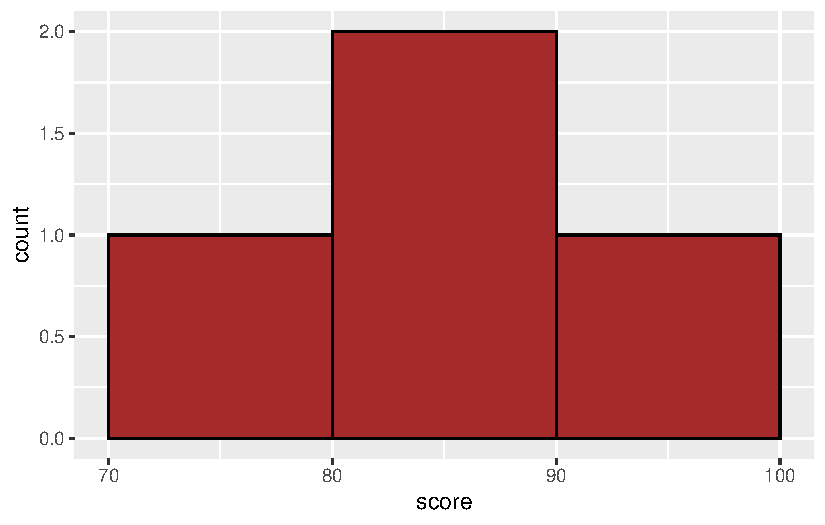
\includegraphics{02-problem-set_files/figure-pdf/3-1.pdf}

}

\end{figure}

\hypertarget{part-e}{%
\subsubsection{Part E}\label{part-e}}

Suppose instead the person who got the 72 did not show up that day to
class, and got a 0 instead. Recalculate the mean and median. What
happened and why?

New set of data: (0, 81, 83, 92).

While the median remains unaffected at 82, the mean becomes much lower
and is now 64.

(0+81+83+92) / 4 = 256 / 4 = 64.

\hypertarget{question-4}{%
\subsection{Question 4}\label{question-4}}

Suppose the probabilities of a visitor to Amazon's website buying 0, 1,
or 2 books are 0.2, 0.4, and 0.4 respectively.

\hypertarget{part-a-2}{%
\subsubsection{Part A}\label{part-a-2}}

Calculate the \emph{expected number} of books a visitor will purchase.

The expected number of purchases is simply the sum of all the
probabilities of purchasing times their respective amount of items
purchased.

(0*0.2) + (1*0.4) + (2*0.4) = 0 + 0.4 + 0.8 = 1.2

\hypertarget{part-b-2}{%
\subsubsection{Part B}\label{part-b-2}}

Calculate the \emph{standard deviation} of book purchases.

To get the standard deviation of these observations, we would first find
the difference between the observations and the mean:

(0-1.2, 1-1.2, 2-1.2) = (-1.2, -0.2, 0.8).

Squaring the differences:

(1.44, 0.04, .64).

Sum the differences:

2.12.

Divide by the sample size minus 1:

2.12 / 3-1 = 2.12 / 2 = 1.06.

And finally take the square root which is roughly equal to 1.029563.

\hypertarget{optional-part-c-bonus}{%
\subsubsection{Optional Part C (Bonus):}\label{optional-part-c-bonus}}

Try doing this in \texttt{R} by making an initial tibble of the data,
and then making new columns to the ``table'' like we did in class.

\begin{Shaded}
\begin{Highlighting}[]
\CommentTok{\# write your code here! }
\NormalTok{amazon }\OtherTok{\textless{}{-}} \FunctionTok{tibble}\NormalTok{(}\AttributeTok{n =} \FunctionTok{c}\NormalTok{(}\DecValTok{0}\NormalTok{,}\DecValTok{1}\NormalTok{,}\DecValTok{2}\NormalTok{),}
                 \AttributeTok{prob =} \FunctionTok{c}\NormalTok{(.}\DecValTok{2}\NormalTok{, .}\DecValTok{4}\NormalTok{, .}\DecValTok{4}\NormalTok{))}
\NormalTok{amazon }\OtherTok{\textless{}{-}}\NormalTok{ amazon }\SpecialCharTok{\%\textgreater{}\%} 
  \FunctionTok{mutate}\NormalTok{(}\AttributeTok{dif =}\NormalTok{ n }\SpecialCharTok{{-}} \FloatTok{1.2}\NormalTok{) }\SpecialCharTok{\%\textgreater{}\%} 
  \FunctionTok{mutate}\NormalTok{(}\AttributeTok{dif\_sqr =}\NormalTok{ dif}\SpecialCharTok{**}\DecValTok{2}\NormalTok{)}

\NormalTok{amazon}
\end{Highlighting}
\end{Shaded}

\begin{verbatim}
# A tibble: 3 x 4
      n  prob   dif dif_sqr
  <dbl> <dbl> <dbl>   <dbl>
1     0   0.2  -1.2  1.44  
2     1   0.4  -0.2  0.0400
3     2   0.4   0.8  0.64  
\end{verbatim}

\hypertarget{question-5}{%
\subsection{Question 5}\label{question-5}}

Scores on the SAT (out of 1600) are approximately normally distributed
with a mean of 500 and standard deviation of 100.

\hypertarget{part-a-3}{%
\subsubsection{Part A}\label{part-a-3}}

What is the probability of getting a score between a 400 and a 600?

Converting both to Z-Scores, we get:

400-500 / 100 = -100/100 = -1

600-500 / 100 = 100/100 = 1.

Since the SAT is normally distributed, we know that 68\% of the
observations, in this case scores, lie between 1 and -1 standard
deviations from the mean. Therefore, there is a 68\% chance to get
between a 400 and a 600 on the SAT.

\hypertarget{part-b-3}{%
\subsubsection{Part B}\label{part-b-3}}

What is the probability of getting a score between a 300 and a 700?

Converting both to Z-Scores, we get:

300-500 / 100 = -200 / 100 = -2

700-500 / 100 = 200 / 100 = 2

Since the SAT is normally distributed, we know that 95\% of the
observations, in this case scores, lie between 2 and -2 standard
deviations from the mean. Therefore, there is a 95\% chance to get
between a 300 and a 700 on the SAT.

\hypertarget{part-c-1}{%
\subsubsection{Part C}\label{part-c-1}}

What is the probability of getting \emph{at least} a 700?

We know that 700 is 2 standard deviations away from the mean from the
last part. And we know that 95\% of the data lies between -2 and 2
standard deviations from the mean. Therefore, 47.5\% of the data lies
between 0 and 2 standard deviations from the mean. And we know that
there is a 50\% to score less than the mean. Therefore, we know that
there is a 97.5\% chance of getting a score up to 2 standard deviations
from the mean. In other words, we know that there is a 97.5\% of getting
at least a 700.\\

\hypertarget{part-d-1}{%
\subsubsection{Part D}\label{part-d-1}}

What is the probability of getting \emph{at most} a 700?

We know that the probability of getting at least of 700 is 97.5\% and
that the area of the probability function is 100\%. Therefore, there
must be a 2.5\% of getting a score better than 700.\\

\hypertarget{part-e-1}{%
\subsubsection{Part E}\label{part-e-1}}

What is the probability of getting exactly a 500?

It is impossible to calculate since we are operating with a continuous
variable(?).

Using calculus we know that the integral of the pdf from 500 to 500 is
0.

\hypertarget{question-6}{%
\subsection{Question 6}\label{question-6}}

Redo problem 5 by using the \texttt{pnorm()} command in \texttt{R}.

\textbf{Hint}: This function has four arguments:

\begin{enumerate}
\def\labelenumi{\arabic{enumi}.}
\tightlist
\item
  the value of the random variable
\item
  the mean of the distribution
\item
  the sd of the distribution
\item
  \texttt{lower.tail} \texttt{TRUE} or \texttt{FALSE}.
\end{enumerate}

\begin{Shaded}
\begin{Highlighting}[]
\CommentTok{\# write your code here! }
\NormalTok{part\_a }\OtherTok{\textless{}{-}}\NormalTok{ (}\FunctionTok{pnorm}\NormalTok{(}\DecValTok{600}\NormalTok{, }\AttributeTok{mean=}\DecValTok{500}\NormalTok{, }\AttributeTok{sd=}\DecValTok{100}\NormalTok{) }\SpecialCharTok{{-}} \FunctionTok{pnorm}\NormalTok{(}\DecValTok{400}\NormalTok{, }\AttributeTok{mean=}\DecValTok{500}\NormalTok{, }\AttributeTok{sd=}\DecValTok{100}\NormalTok{))}
\NormalTok{part\_a}
\end{Highlighting}
\end{Shaded}

\begin{verbatim}
[1] 0.6826895
\end{verbatim}

\begin{Shaded}
\begin{Highlighting}[]
\NormalTok{part\_b }\OtherTok{\textless{}{-}}\NormalTok{ (}\FunctionTok{pnorm}\NormalTok{(}\DecValTok{700}\NormalTok{, }\AttributeTok{mean=}\DecValTok{500}\NormalTok{, }\AttributeTok{sd=}\DecValTok{100}\NormalTok{) }\SpecialCharTok{{-}} \FunctionTok{pnorm}\NormalTok{(}\DecValTok{300}\NormalTok{, }\AttributeTok{mean=}\DecValTok{500}\NormalTok{, }\AttributeTok{sd=}\DecValTok{100}\NormalTok{))}
\NormalTok{part\_b}
\end{Highlighting}
\end{Shaded}

\begin{verbatim}
[1] 0.9544997
\end{verbatim}

\begin{Shaded}
\begin{Highlighting}[]
\NormalTok{part\_c }\OtherTok{\textless{}{-}} \FunctionTok{pnorm}\NormalTok{(}\DecValTok{700}\NormalTok{, }\AttributeTok{mean=}\DecValTok{500}\NormalTok{, }\AttributeTok{sd=}\DecValTok{100}\NormalTok{)}
\NormalTok{part\_c}
\end{Highlighting}
\end{Shaded}

\begin{verbatim}
[1] 0.9772499
\end{verbatim}

\begin{Shaded}
\begin{Highlighting}[]
\NormalTok{part\_d }\OtherTok{\textless{}{-}} \FunctionTok{pnorm}\NormalTok{(}\DecValTok{700}\NormalTok{, }\AttributeTok{mean=}\DecValTok{500}\NormalTok{, }\AttributeTok{sd=}\DecValTok{100}\NormalTok{, }\AttributeTok{lower.tail=}\ConstantTok{FALSE}\NormalTok{)}
\NormalTok{part\_d}
\end{Highlighting}
\end{Shaded}

\begin{verbatim}
[1] 0.02275013
\end{verbatim}

\begin{Shaded}
\begin{Highlighting}[]
\NormalTok{part\_e }\OtherTok{\textless{}{-}} \FunctionTok{pnorm}\NormalTok{(}\DecValTok{500}\NormalTok{, }\AttributeTok{mean=}\DecValTok{500}\NormalTok{, }\AttributeTok{sd=}\DecValTok{100}\NormalTok{) }\SpecialCharTok{{-}} \FunctionTok{pnorm}\NormalTok{(}\DecValTok{500}\NormalTok{, }\AttributeTok{mean=}\DecValTok{500}\NormalTok{, }\AttributeTok{sd=}\DecValTok{100}\NormalTok{)}
\NormalTok{part\_e}
\end{Highlighting}
\end{Shaded}

\begin{verbatim}
[1] 0
\end{verbatim}

\hypertarget{knit-and-submit}{%
\section{Knit and Submit!}\label{knit-and-submit}}

When you are done, click the \textbf{Render} button. Based on the
current \texttt{yaml} header \texttt{format:\ html}, this will currently
produce an html webpage, which should automatically open for your
review.

Notice in the \textbf{Files} pane in R Studio (by default, the lower
right one), there should now be a document called
\texttt{01-problem-set.html} (or if you changed the filename) ending in
\texttt{.html}. This is the webpage, so you can find this file on your
computer (or download it from Rstudio.cloud with by clicking on the
checkmark box in front of the file in the Files page and then going to
\texttt{More\ -\textgreater{}\ Export...} to download the file to your
computer) and send this file.

If you want to make a PDF, install the package ``tinytex'' and run the
following code to install a LaTeX distribution:

Then delete the lines in the \texttt{yaml} header that say
\texttt{format:\ html:\ self-contained:\ TRUE}, and add a simple line
that says \texttt{format:\ pdf} . Clicking \textbf{Render} will now
produce a PDF, show it, and save it as a new file in the Files pane.

Either way, send me your output file, \texttt{html} or \texttt{pdf} (or,
if you like, \texttt{word}) so long as it shows the input and output
code of every chunk. I have set it by default to do this, with
\texttt{echo:\ true} in the \texttt{yaml} header.

Don't forget to add your name to the \texttt{author} part of the header!



\end{document}
